\documentclass{article}
    \usepackage{float}
    \usepackage{textcomp}
    \usepackage{graphicx}
    \usepackage{booktabs}
    \usepackage{color}
    \usepackage{verbatim}
    \usepackage{listings}
    \usepackage{underscore}
    \usepackage{amsmath}
    \usepackage{amssymb}
    %\usepackage{showkeys}
    %\usepackage{float} % here for H placement parameter
    \usepackage{flafter} 
    \setcounter{secnumdepth}{5}
    \usepackage[bookmarks=true]{hyperref}
    \author{\textbf{Marco Bissessur}} 
    \date{23 Giugno 2018}
    \title{ITIS G. Feltrinelli
        \\A.A. 2017\@-\@2018
        \\Documentazione tesina maturità \\ \textbf{Badminton Clubs}
      } 
        \hypersetup{pdftitle={Documentazione},    % title
        pdfauthor={Marco Bissessur},                     % author
        pdfsubject={tesina},                        % subject of the document
        colorlinks=true,       % false: boxed links; true: colored links
        linkcolor=blue,       % color of internal links
        citecolor=blue,       % color of links to bibliography
        filecolor=black,        % color of file links
        urlcolor=blue,        % color of external links
       }
    \begin{document}
    \maketitle
    \begin{center}
        
\includegraphics[width=7cm]{logofeltrinelli}
    \end{center}
    \clearpage
    {\hypersetup{hidelinks}\tableofcontents}
    \clearpage
    
    \section{Introduzione}

    \section{Obiettivo}
%L'Obiettivo principale di Badminton Clubs è di aiutare gli utenti a organizzare tornei tra amici o con altri utenti, formare gruppi di amici o incontrare nuove persone attraverso club e  
L'Obiettivo principale di Badminton Clubs è di creare un social network che permette agli utenti di organizzare e gestire tornei tra di loro, nello specifico voglio creare un prodotto che possa:
\begin{itemize}
    \item Permettere agli utenti di inviare richieste di amicizia, accettarle e visuallizare gli amici
    \item Permettere agli utenti di creare tornei con nome, descrizione, numero di partecipanti, tipo di torneo (singolo, doppio) e il sesso dei partecipanti. Gestirli e organizzare i turni.
    \item Permettere agli utenti di creare club e fare gruppi tra di loro.
    \item Permettere agli utenti  di visuallizare i club in base ad una classifica in base al loro punteggio.
    \item Permettere di visualizzare gli utenti iscritti e gli ultimi tornei creati
\end{itemize}
\section{Requisiti funzionali}

    \section{Tecnologia utilizzata}
    \subsection{Front end}
    \subsubsection{Linguaggi}
 I linguaggi Front end che ho utilizzato sono:
 \begin{itemize}
    \item HTML per creare la struttura base delle pagine dell'applicazione
    \item CSS per modellare la pagina e renderla responsive 
    \item JAVASCRIPT per creare animazioni, e soprattutto per la creazione dinamica
    dell'albero che rappresenta i vari match di un torneo.
  \end{itemize}
    \subsection{Back end}
    \subsubsection{Linguaggi}
Per programmare il back end ho utilizzato il linguaggio PHP, per creare contenuto
dinamico nelle pagine, i cui dati sono presi tramite query
dal database MySql.
\subsubsection{Hosting}
L'applicazione è stata pubblicata sul dominio .... affittato
da Aruba srl, la gestione del database è avvenuta come per il 
database locale di MAMP.



\subsection{Database}
    Questo è lo schema UML della struttura del database progettato con MySql
    \begin{center}
        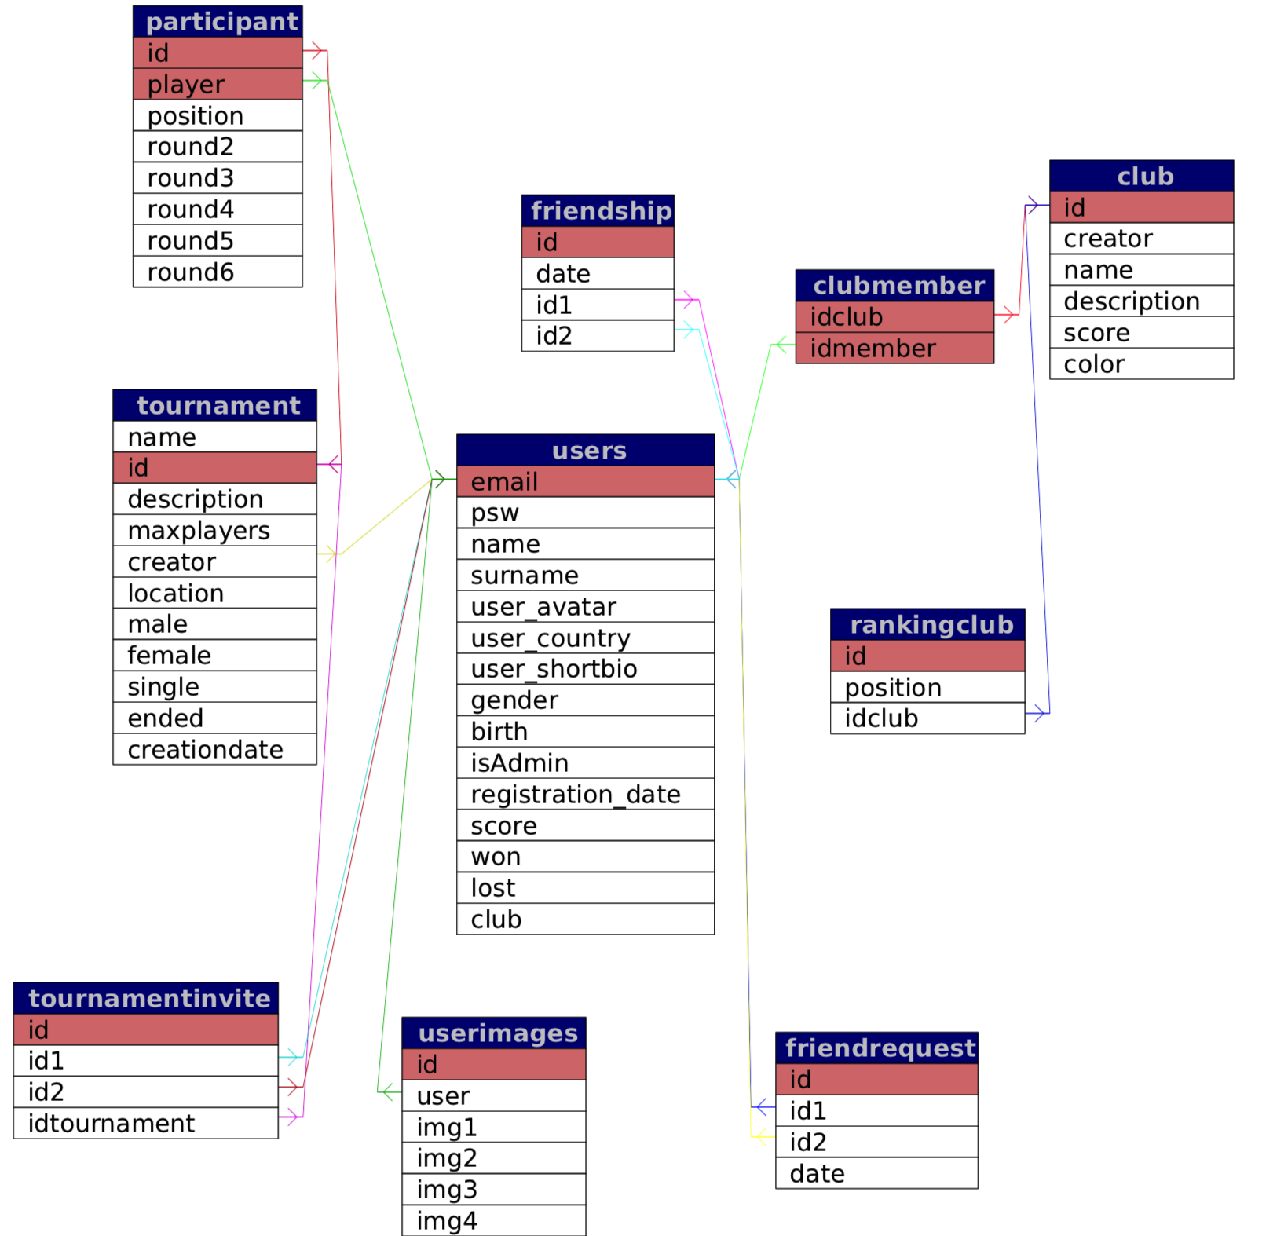
\includegraphics[width=15cm]{images/schemapng}
    \end{center}
    \subsubsection{Users}
    \begin{center}
        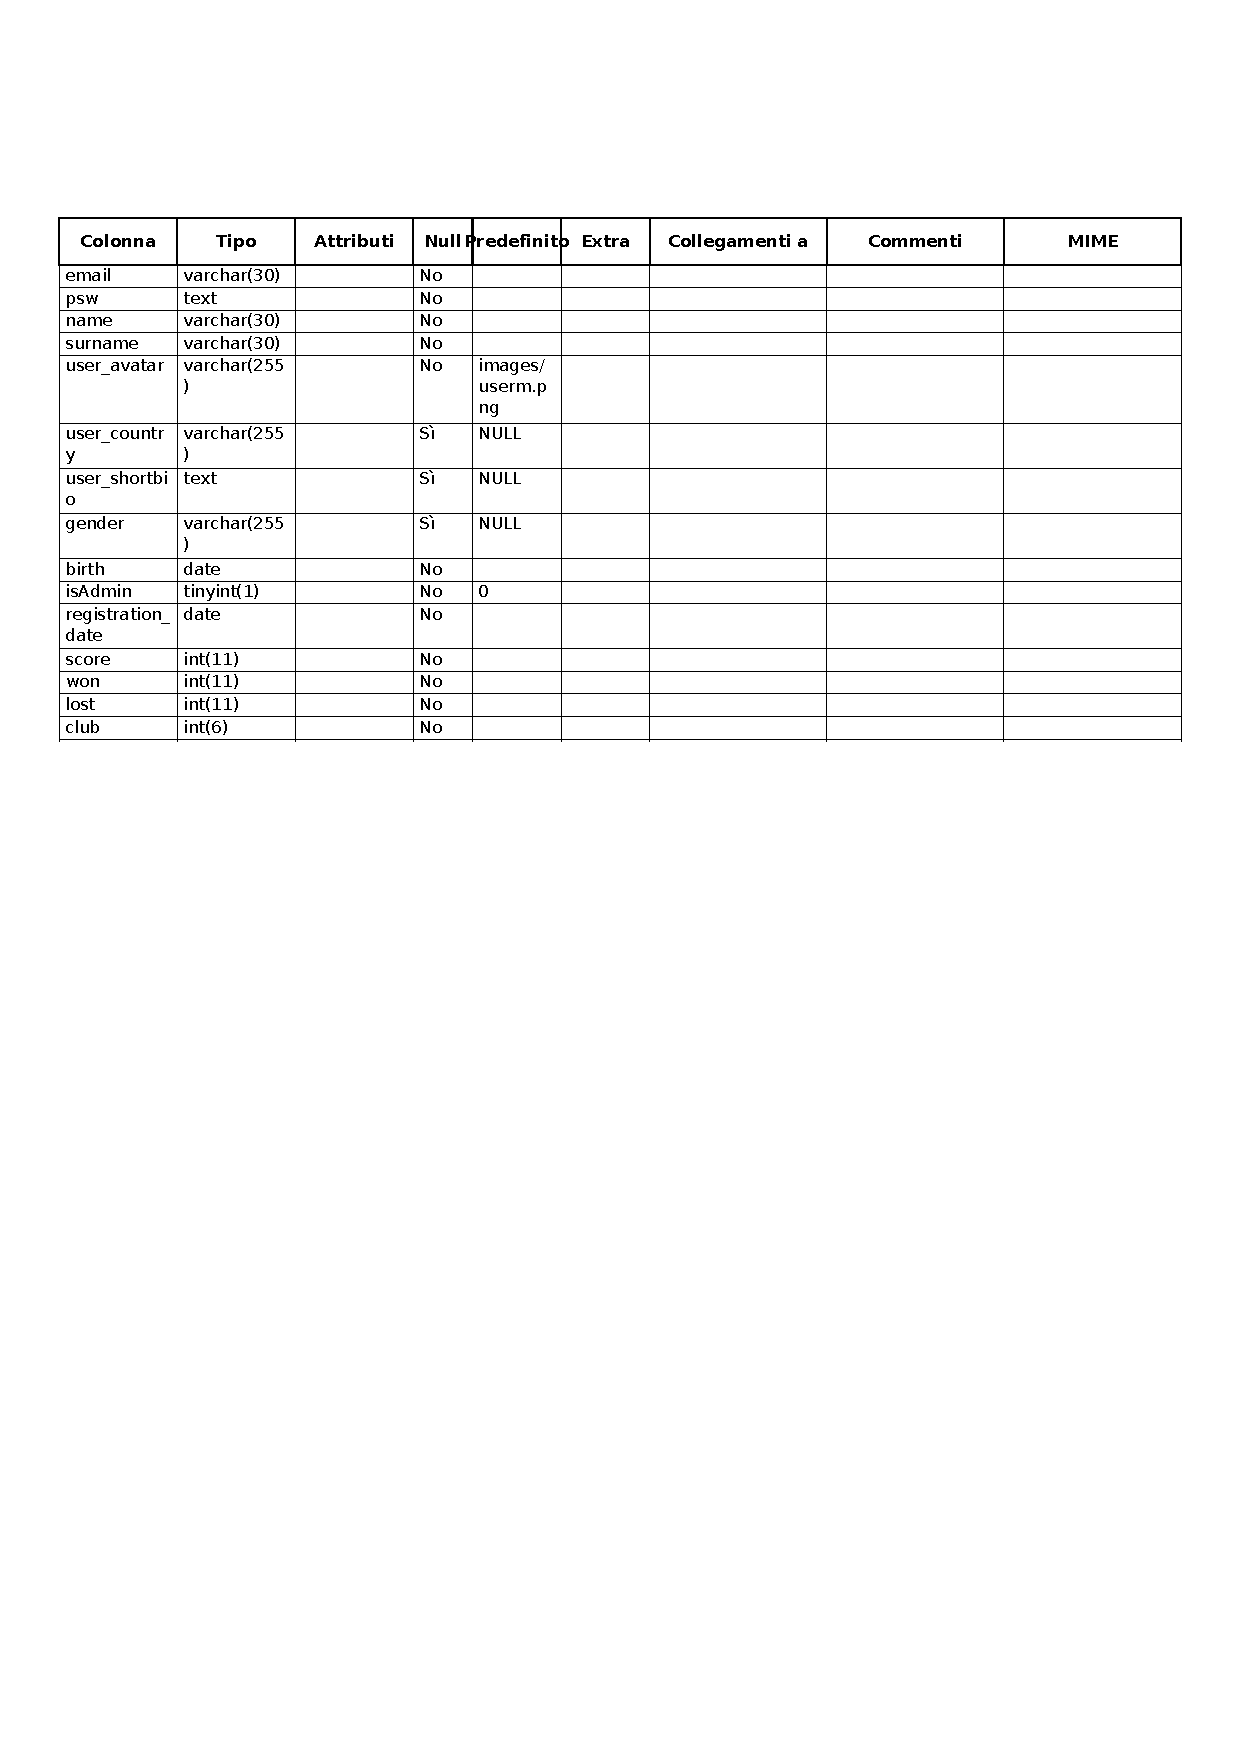
\includegraphics[width=15cm]{images/users}
    \end{center}
    \subsubsection{Club}
    \begin{center}
        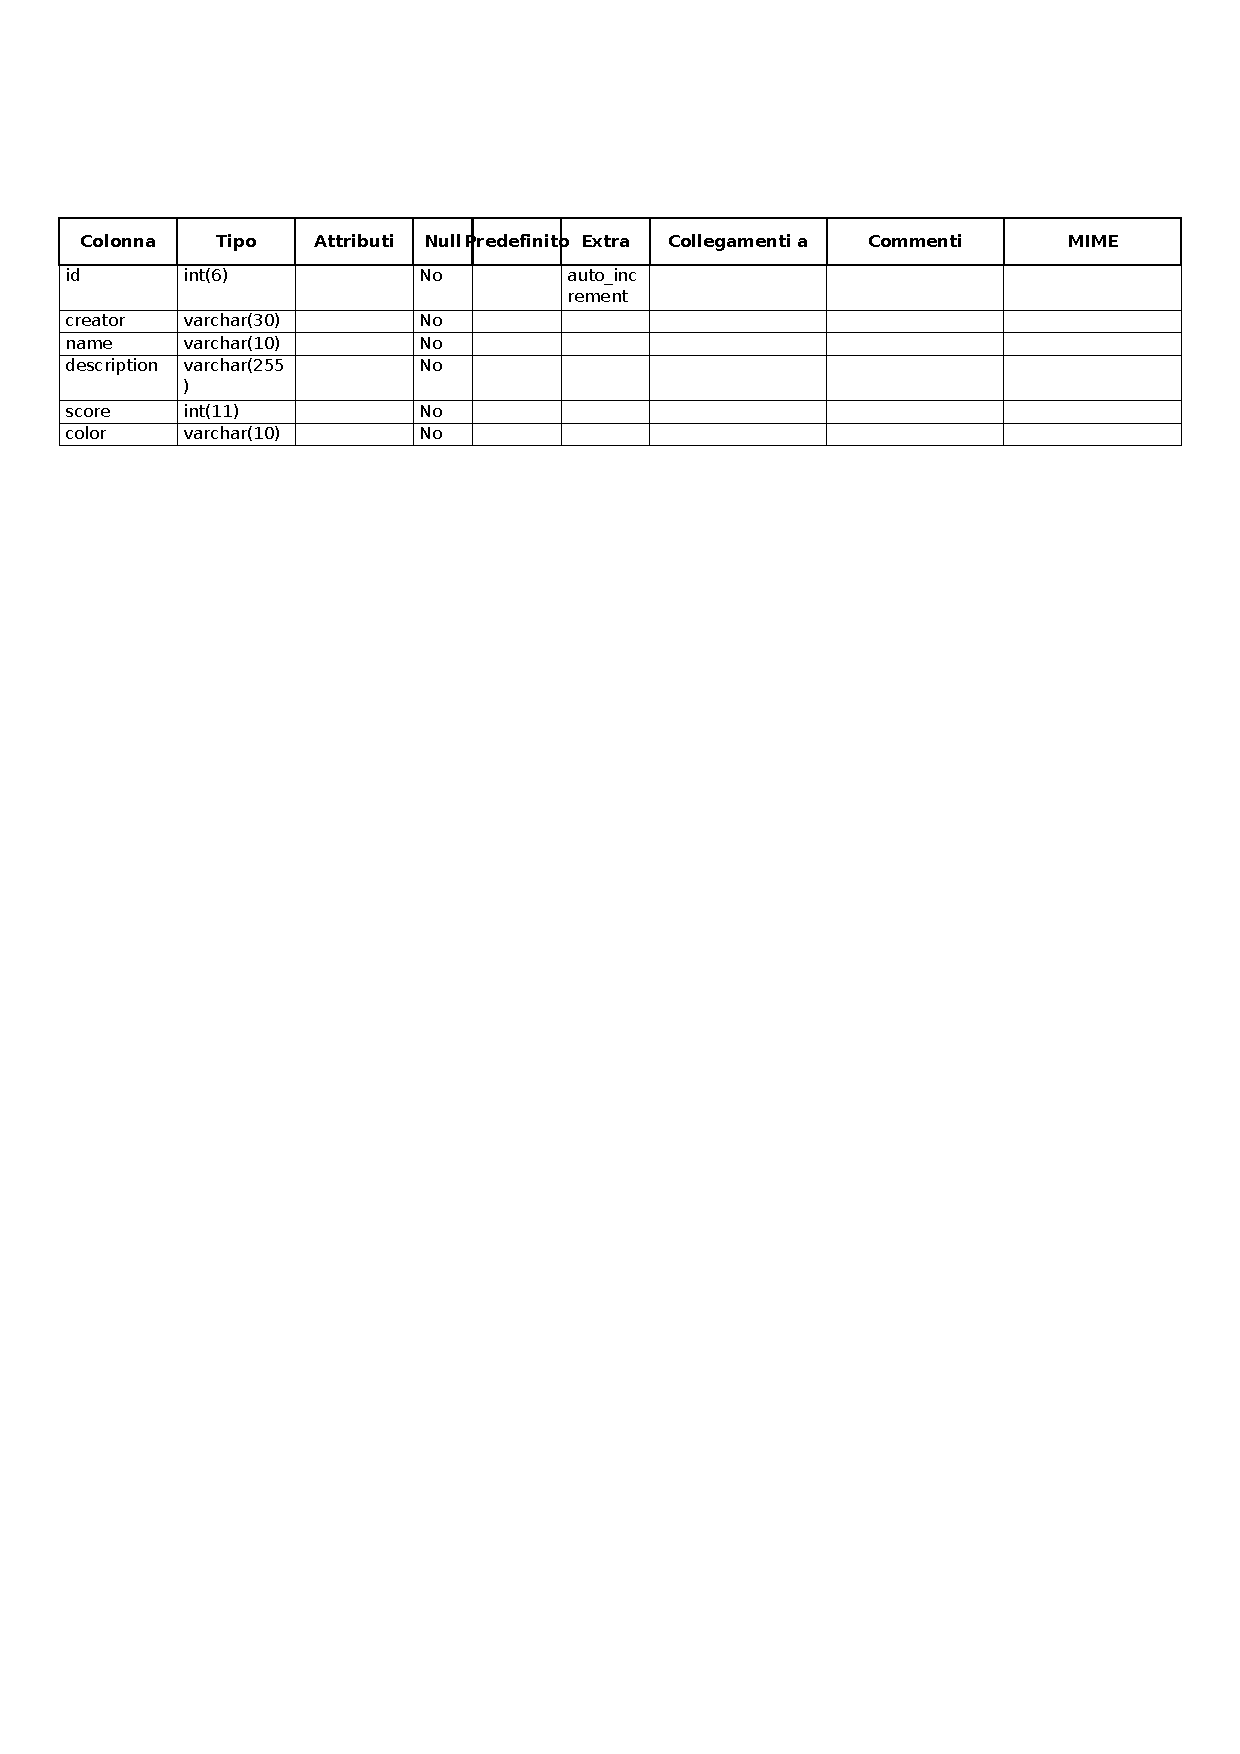
\includegraphics[width=15cm]{images/club}
    \end{center} 
    \subsubsection{Club Ranking}
    \begin{center}
        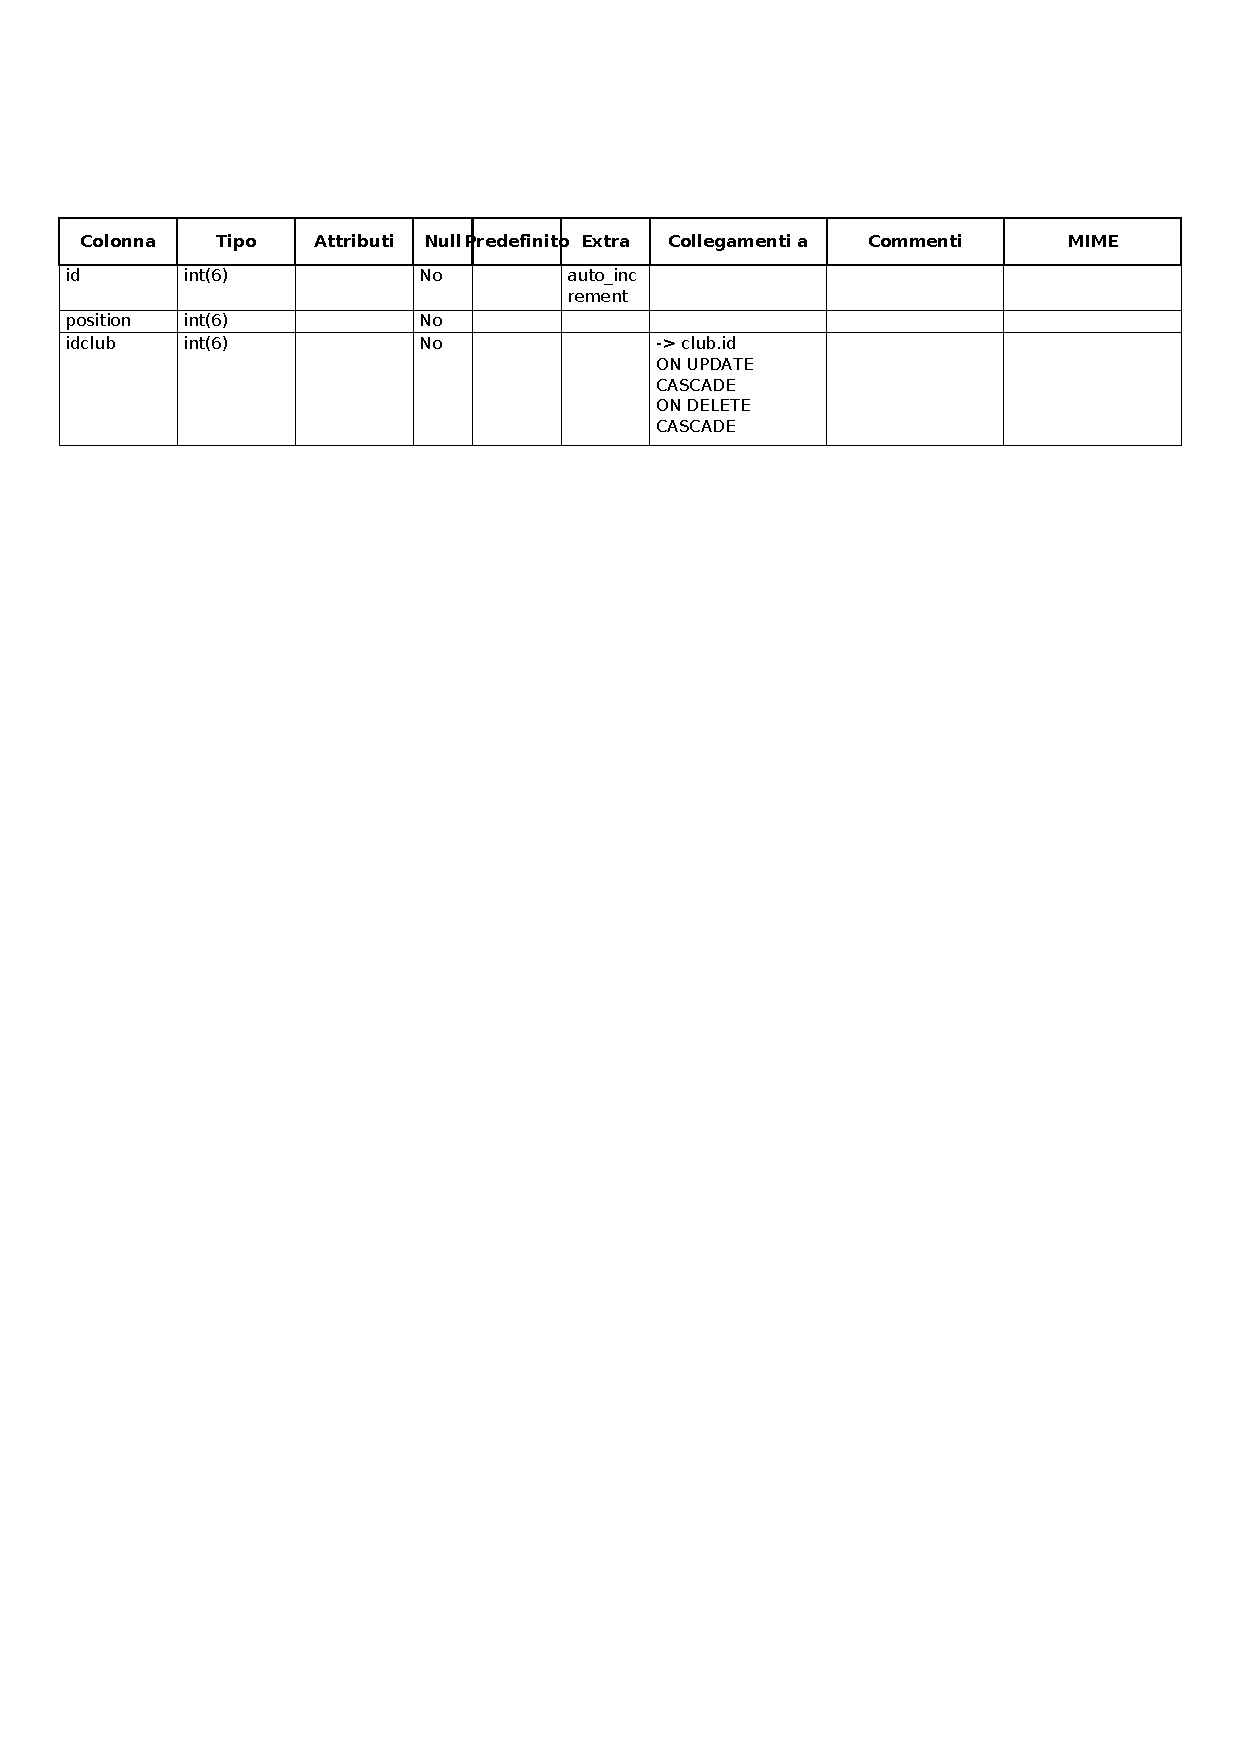
\includegraphics[width=15cm]{images/rankingclub}
    \end{center}
    \subsubsection{User images}
    \begin{center}
        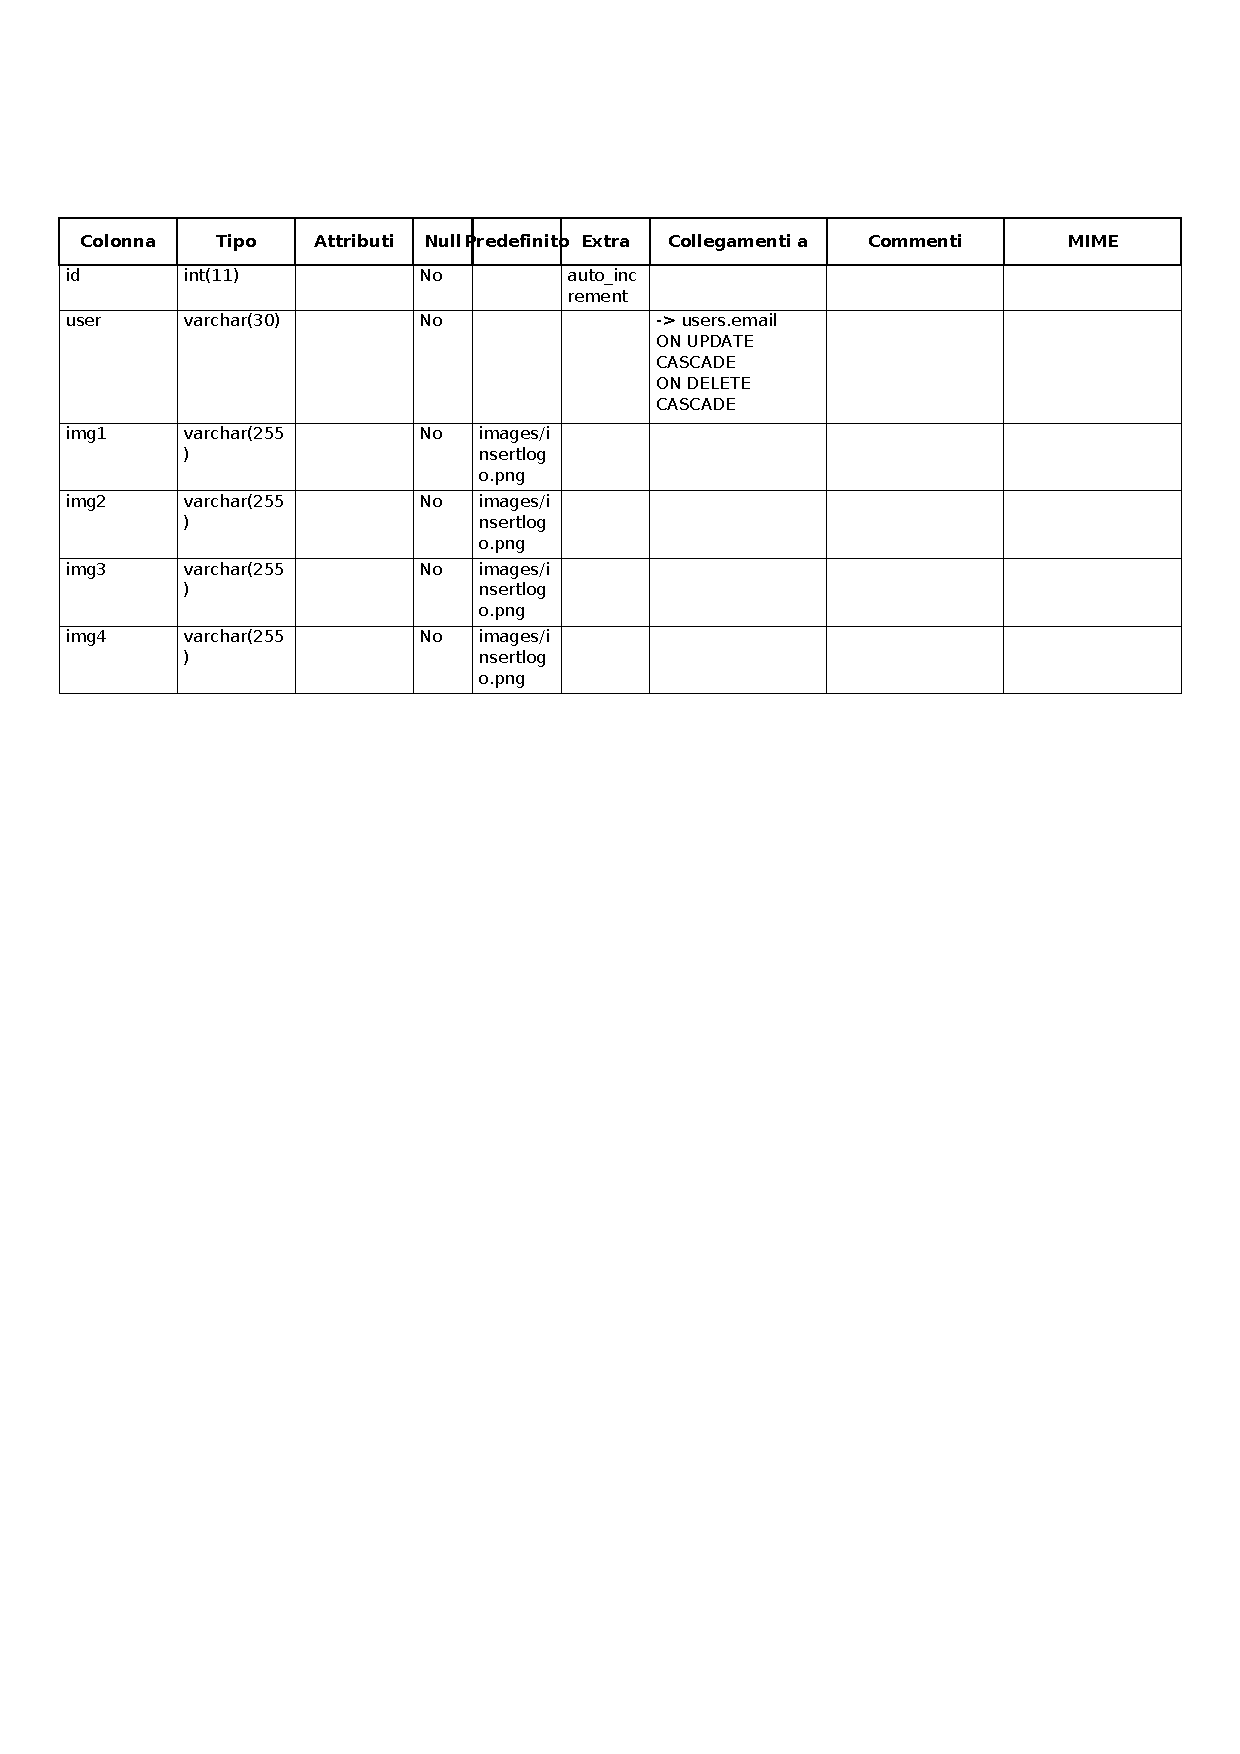
\includegraphics[width=15cm]{images/userimages}
    \end{center}
    \subsubsection{Tournament}
    \begin{center}
        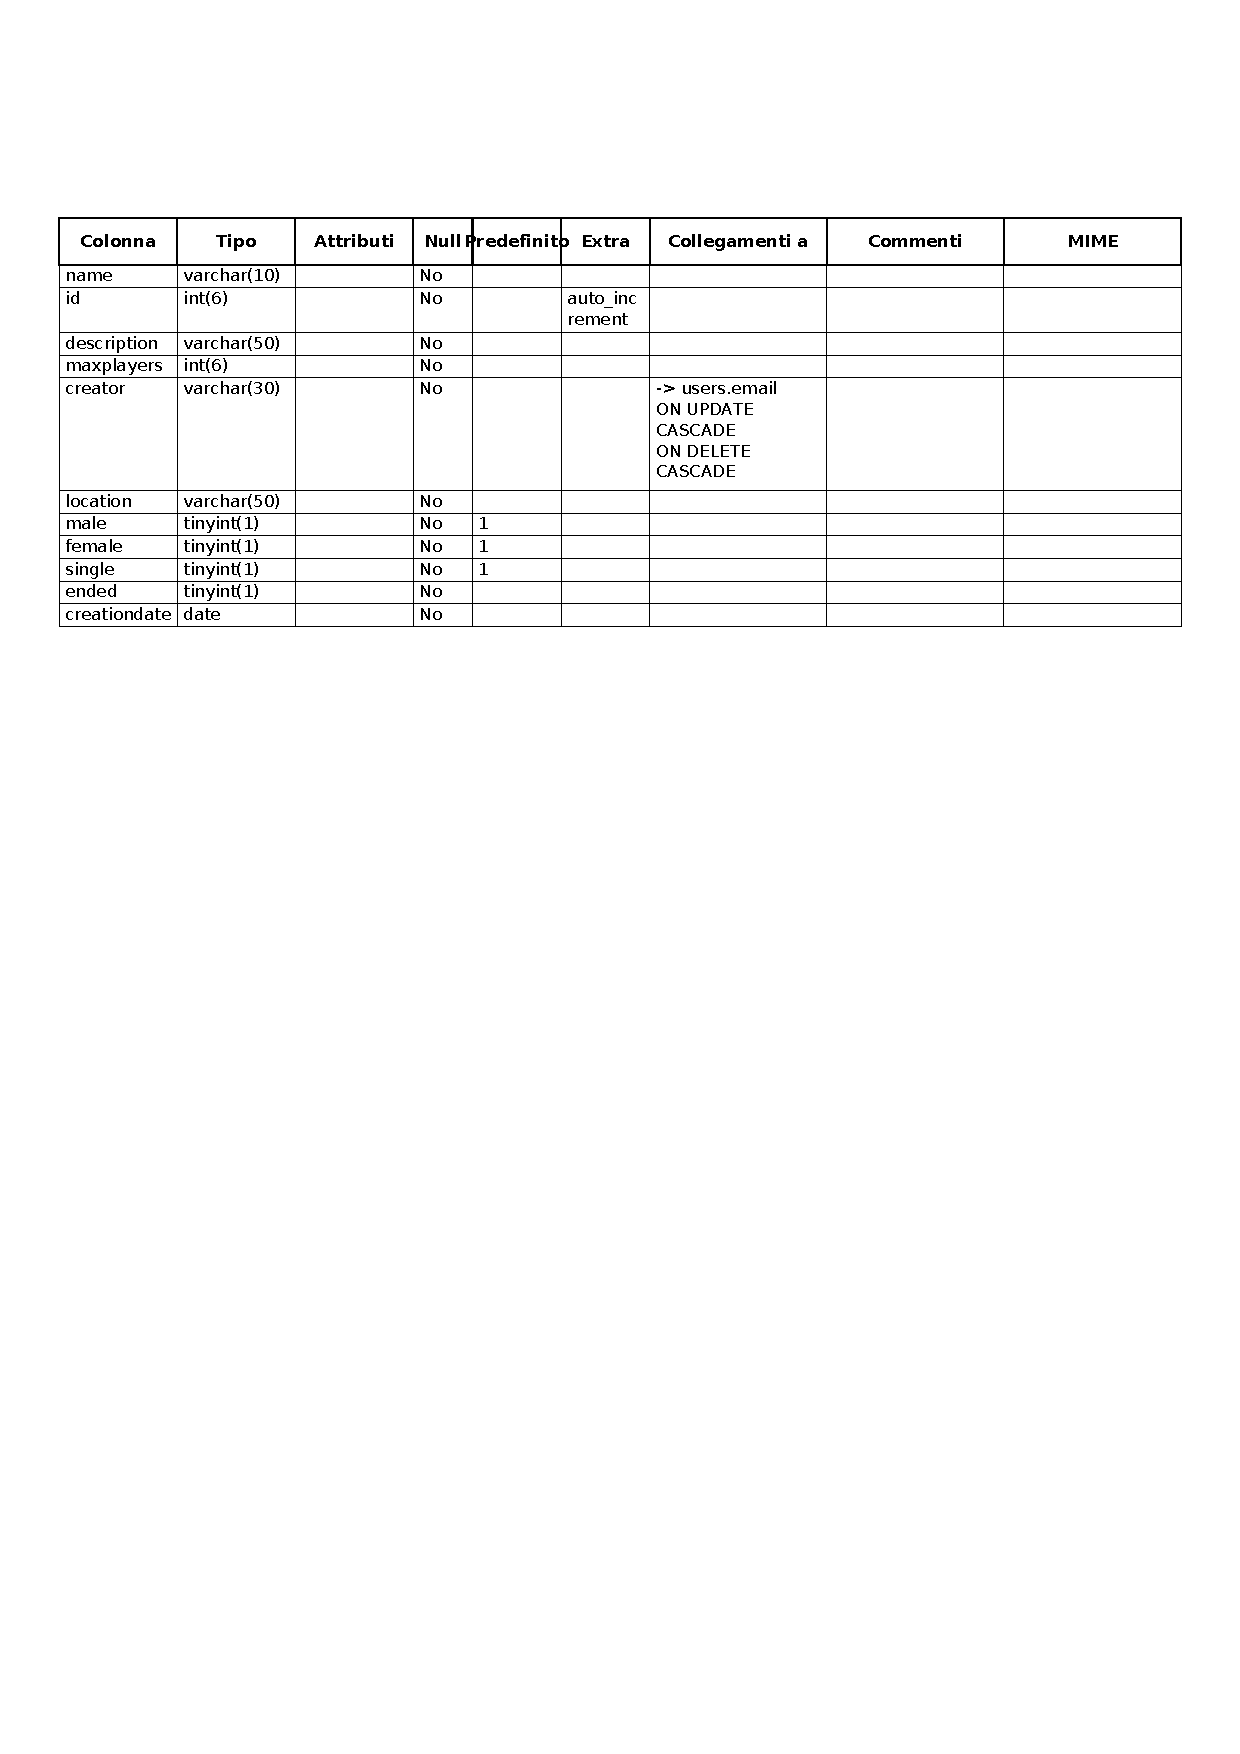
\includegraphics[width=15cm]{images/tournament}
    \end{center}
    \subsubsection{Participant}
    \begin{center}
        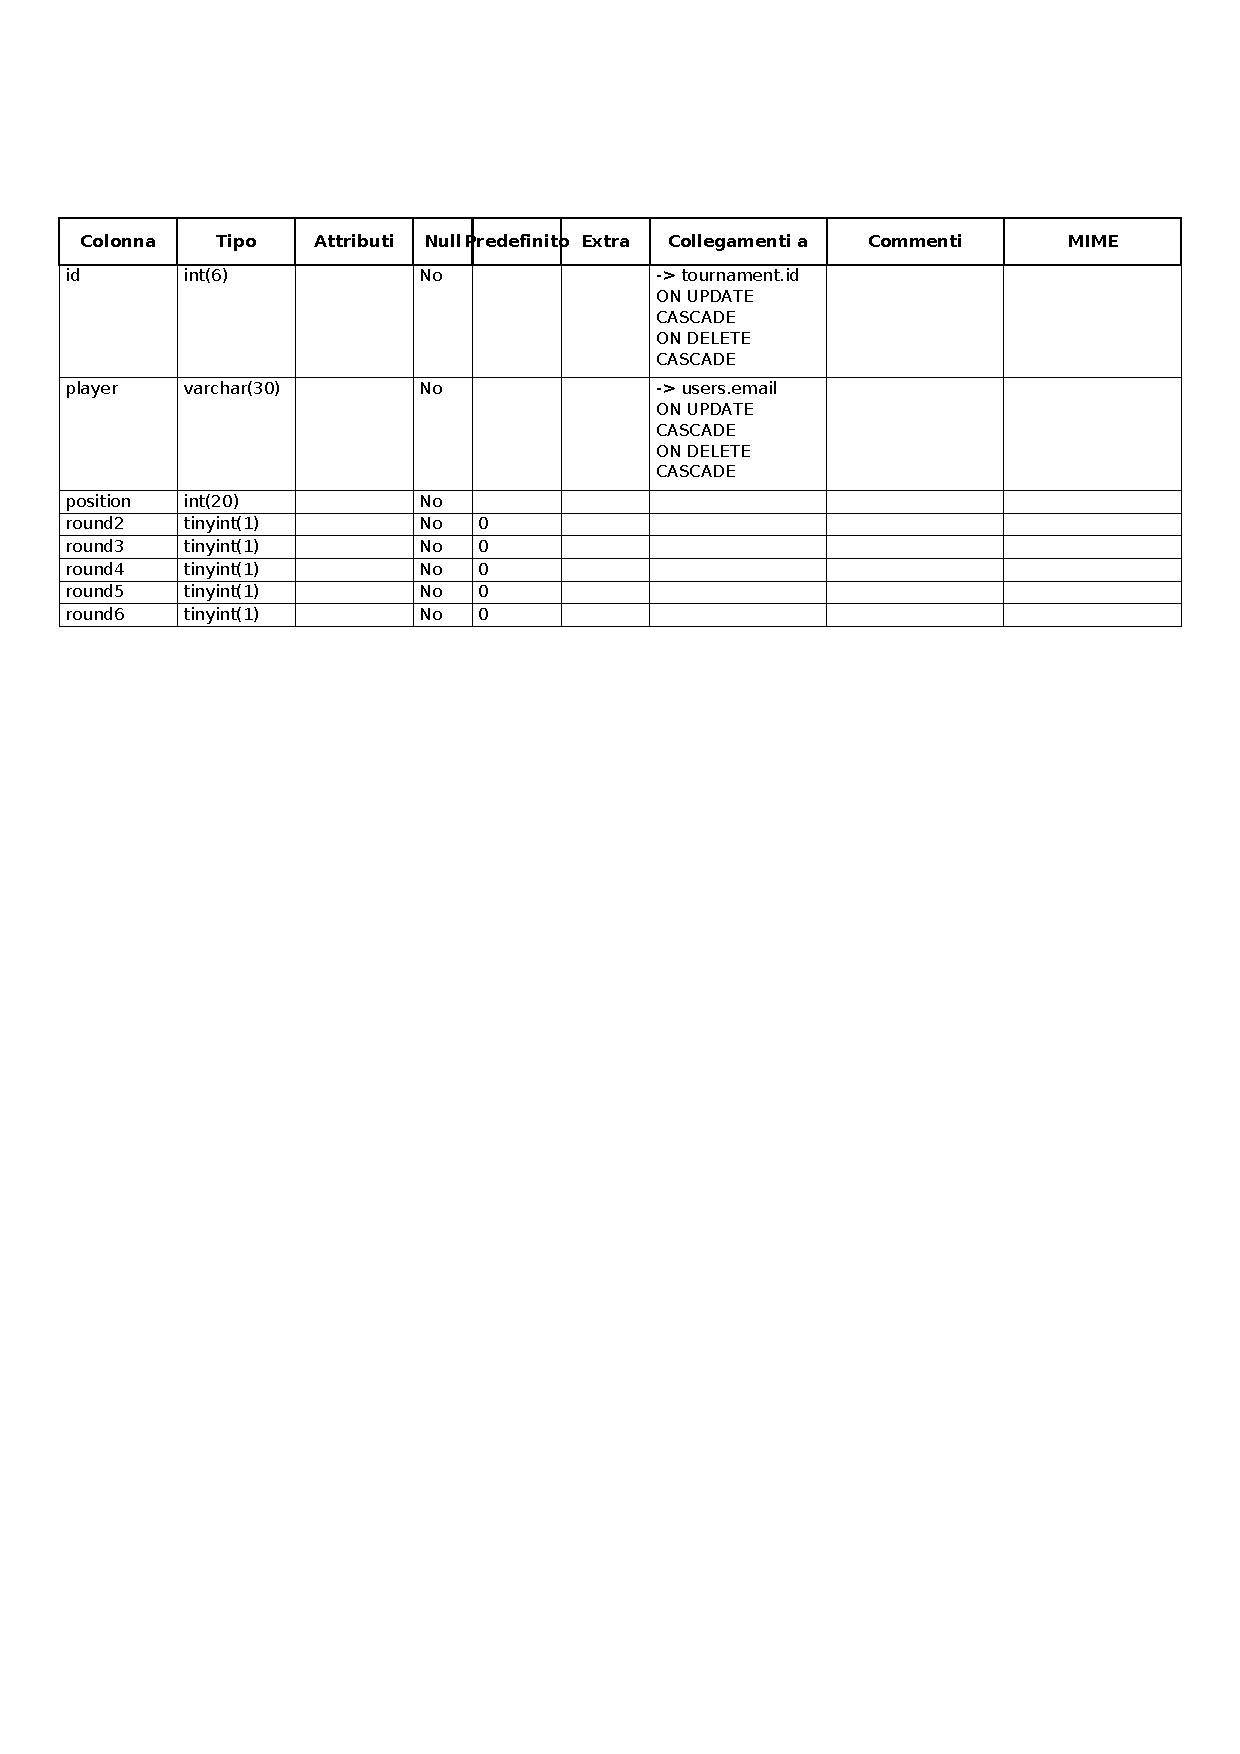
\includegraphics[width=15cm]{images/participant}
    \end{center}
    \subsubsection{Friendship}
    \begin{center}
        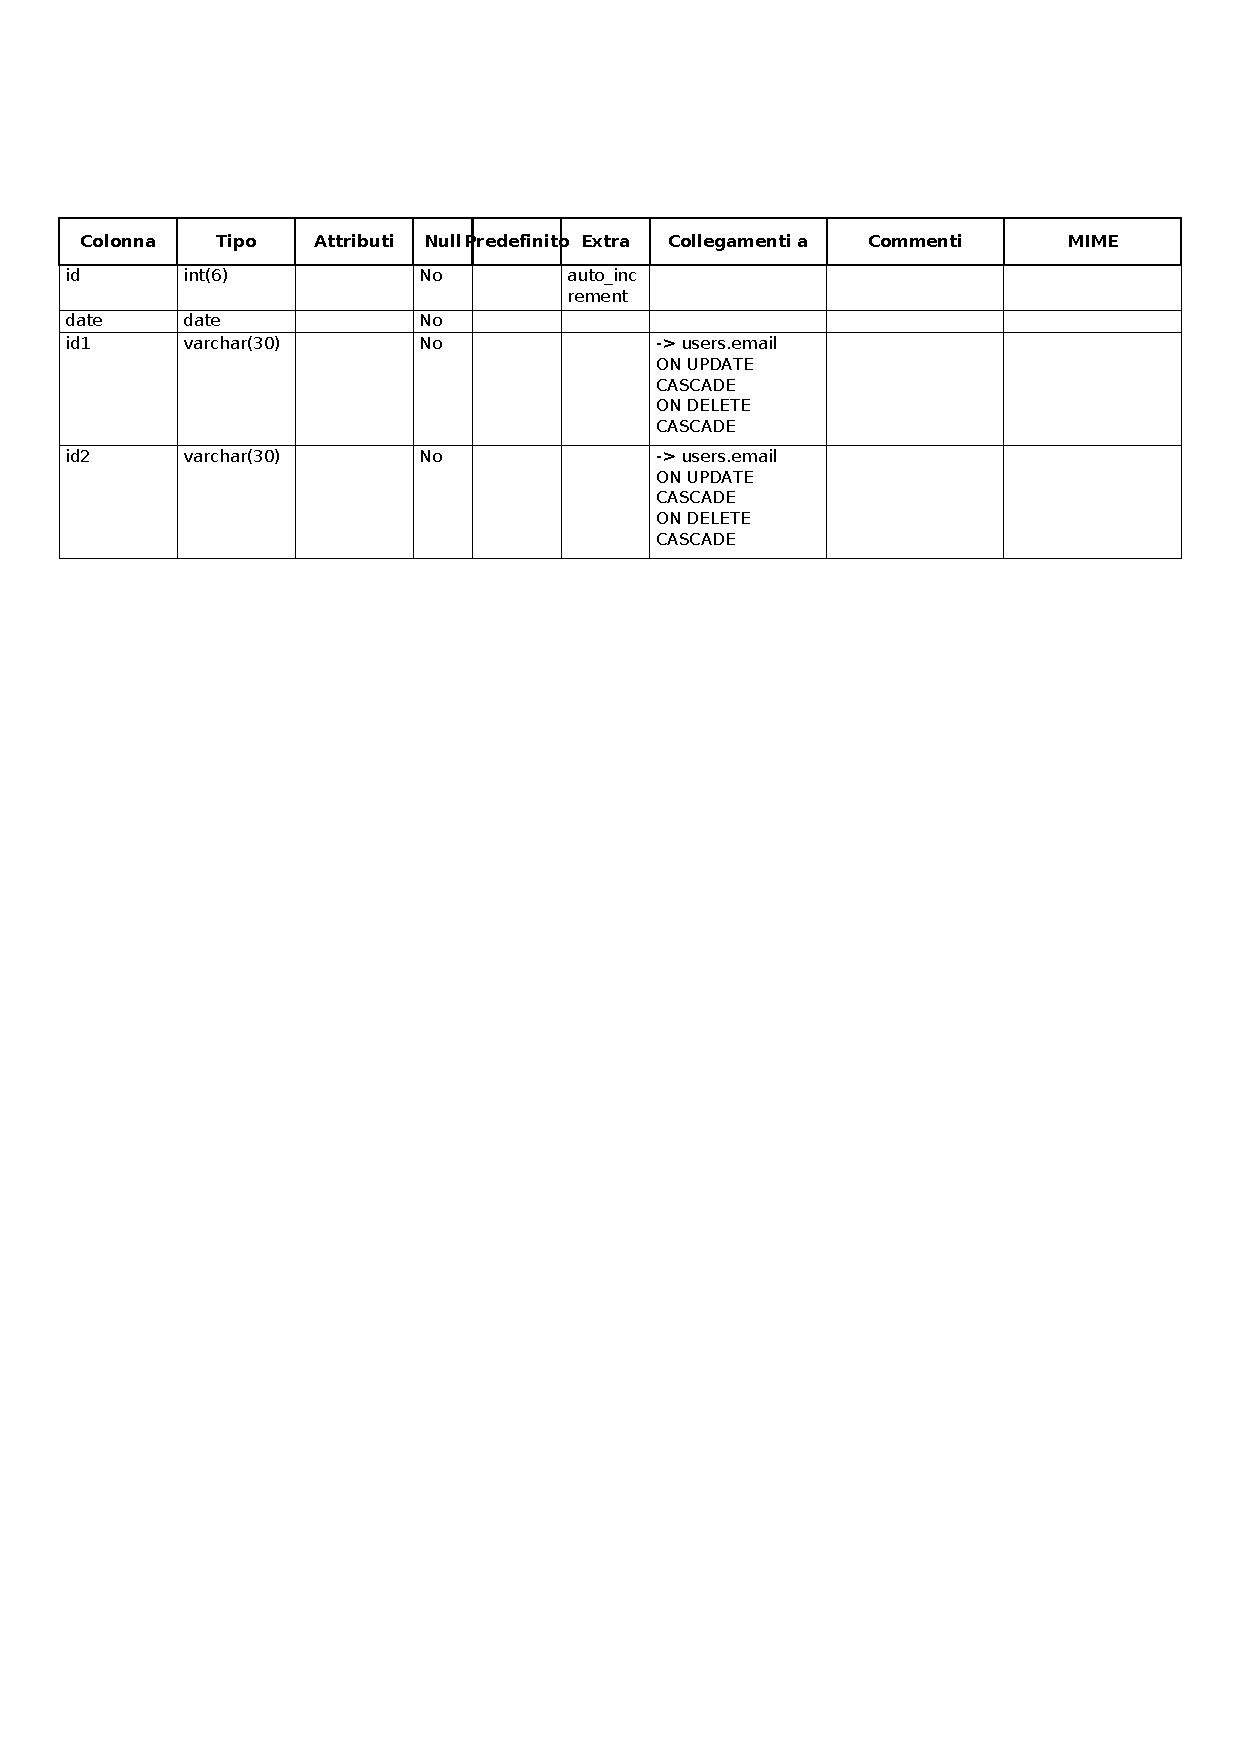
\includegraphics[width=15cm]{images/friendship}
    \end{center}
    \subsubsection{Friend Request}
    \begin{center}
        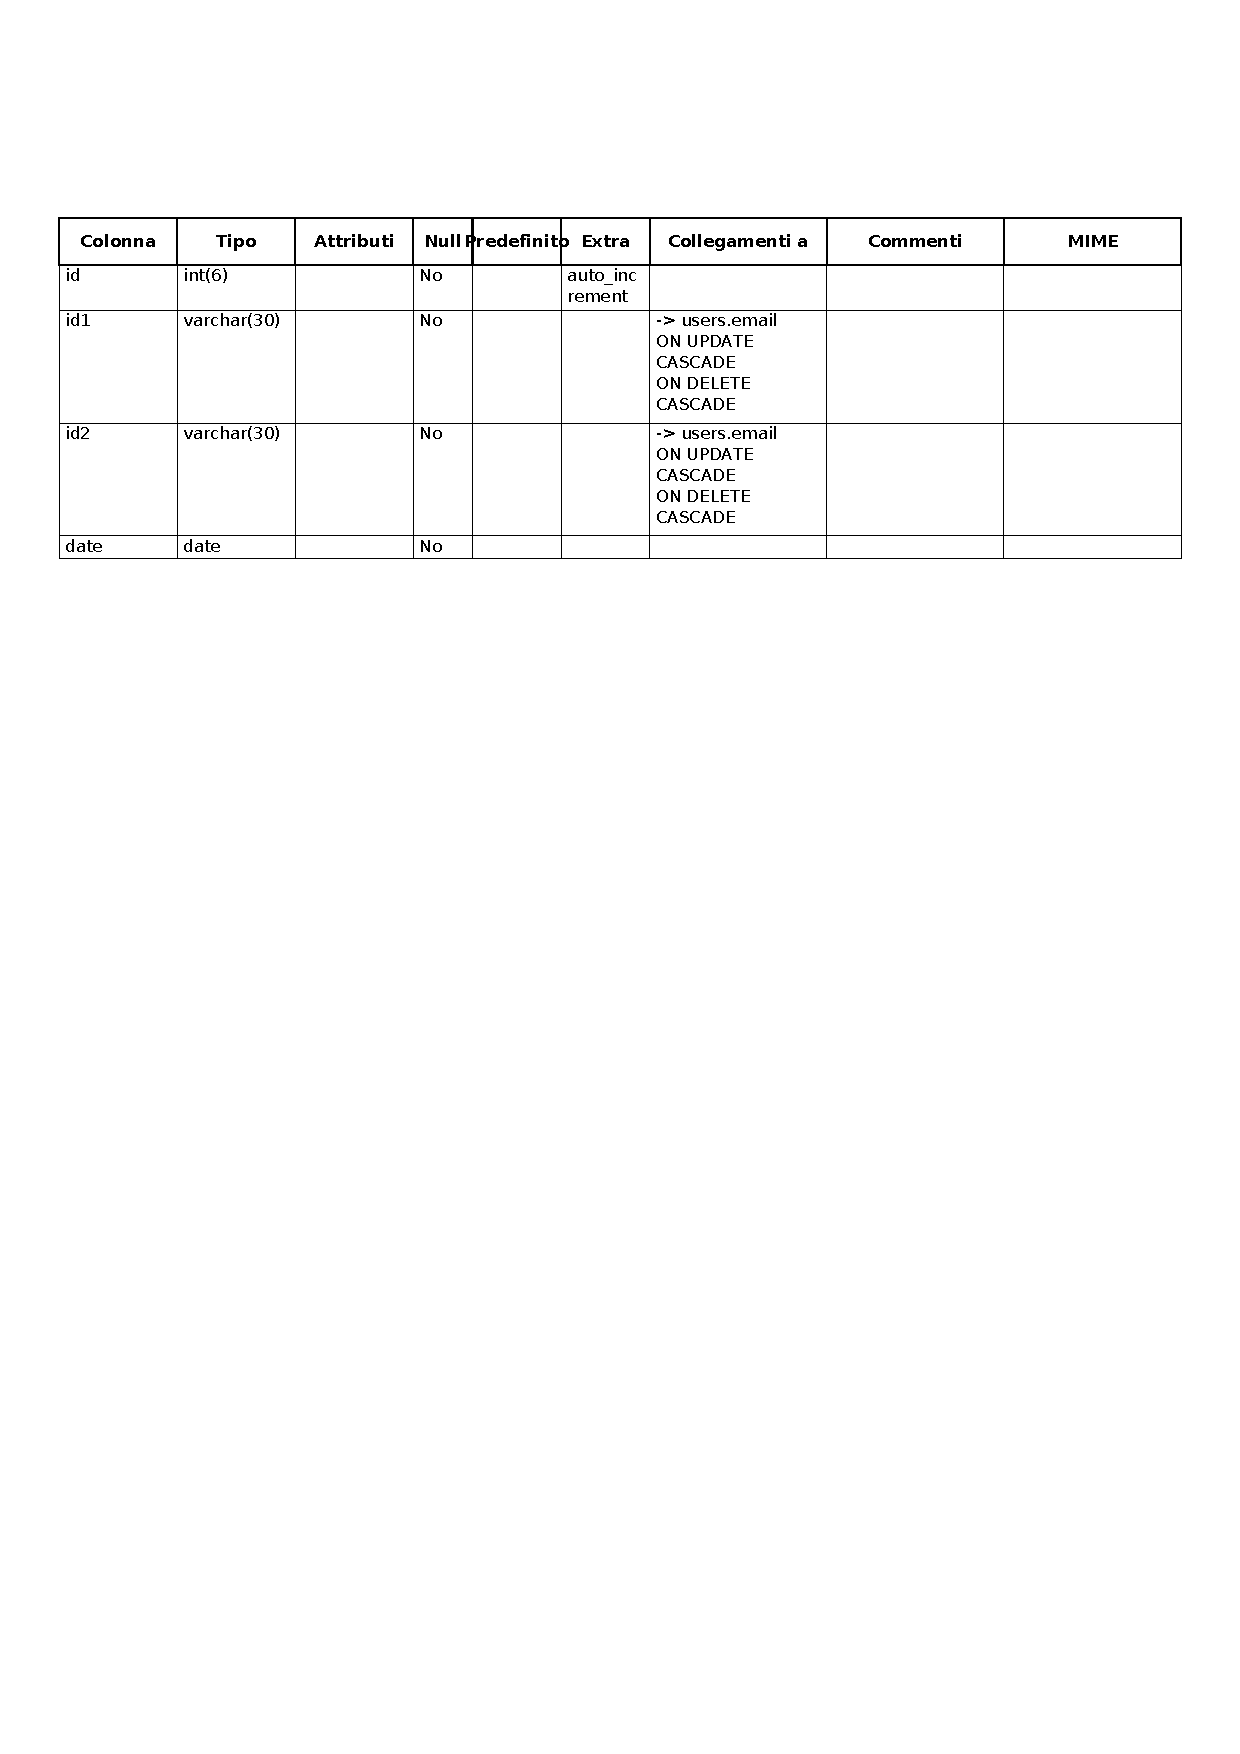
\includegraphics[width=15cm]{images/friendrequest}
    \end{center}
    \subsubsection{Club member}
    \begin{center}
        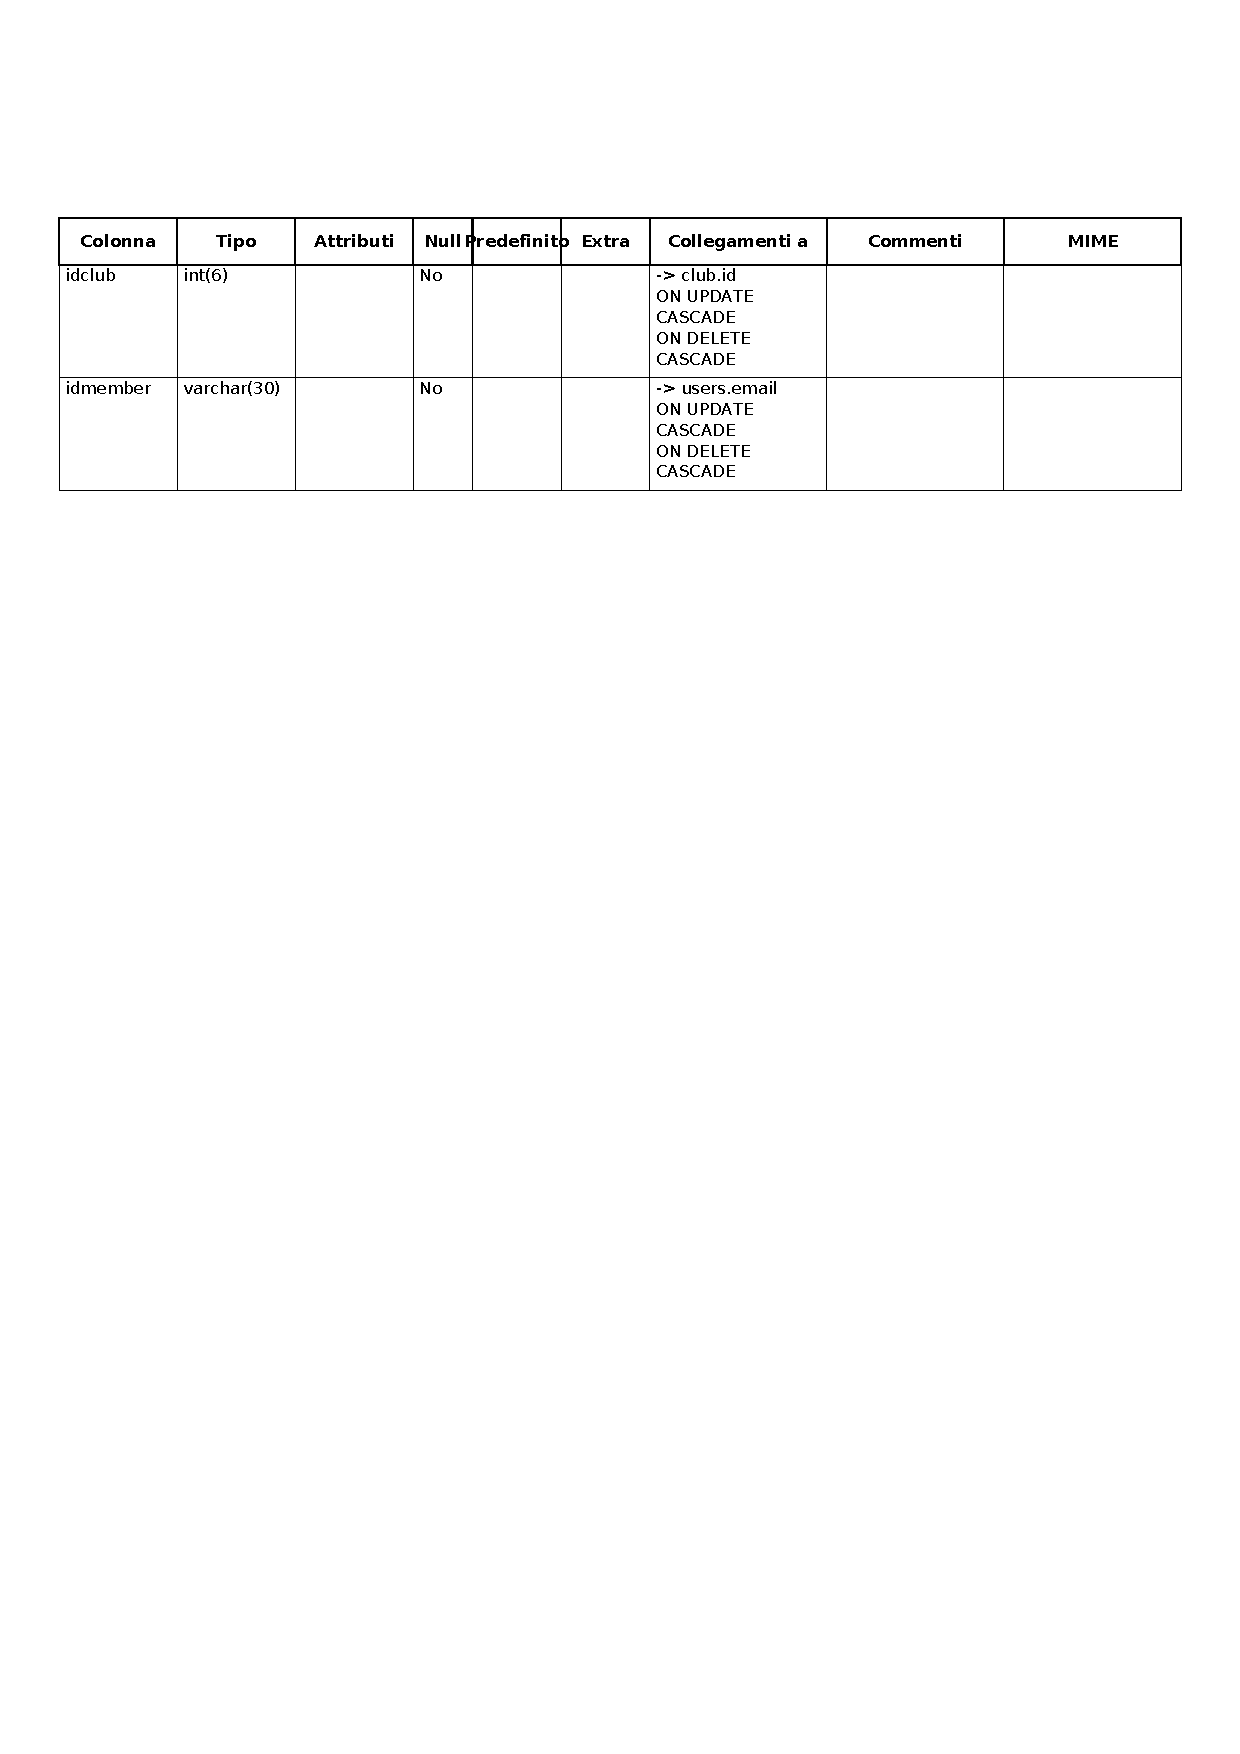
\includegraphics[width=15cm]{images/clubmember}
    \end{center}

    \section{Use cases}
    tabelle con omini
    spiegazione delle tabelle, es. come l'admin del torneo gestisce il torneo

    \section{UX user experience}
    navigazione pagine 
   




    \section{Workflow}

Per fare il social network ho utilizzato MAMP per lavorare in locale sul mio computer, L'IDE che ho utilizzato è Brackets che ho usato per programmare le pagine front e back end. Ho utilizzanto git come Version Control System per gestire il workflow, infine ho pubblicato l'applicazione su un dominio online 
(\href{https://www.marcobissessur.it}{Badminton Clubs}) \\
Per la Documentazione ho utlizzato il linguaggio Latex e Visual Studio Code come ide.
    

    
    
    \end{document}